 \documentclass{sigchi}

\usepackage{balance}       % to better equalize the last page
\usepackage{graphics}      % for EPS, load graphicx instead 
\usepackage[T1]{fontenc}   % for umlauts and other diaeresis
\usepackage{txfonts}
\usepackage{mathptmx}
\usepackage[pdflang={en-US},pdftex]{hyperref}
\usepackage{color}
\usepackage{booktabs}
\usepackage{textcomp}


% Some optional stuff you might like/need.
\usepackage{microtype}        % Improved Tracking and Kerning
% \usepackage[all]{hypcap}    % Fixes bug in hyperref caption linking
\usepackage{ccicons}          % Cite your images correctly!
% \usepackage[utf8]{inputenc} % for a UTF8 editor only


\usepackage{todonotes}
\def\plaintitle{Physics 111 : Optical Pumping}
\def\plainauthor{Jung Lin Lee \\[Partner: Xiyue Wang]}
\makeatletter
\def\url@leostyle{%
  \@ifundefined{selectfont}{
    \def\UrlFont{\sf}
  }{
    \def\UrlFont{\small\bf\ttfamily}
  }}
\makeatother
\urlstyle{leo}

% To make various LaTeX processors do the right thing with page size.
\def\pprw{8.5in}
\def\pprh{11in}
\special{papersize=\pprw,\pprh}
\setlength{\paperwidth}{\pprw}
\setlength{\paperheight}{\pprh}
\setlength{\pdfpagewidth}{\pprw}
\setlength{\pdfpageheight}{\pprh}

% Make sure hyperref comes last of your loaded packages, to give it a
% fighting chance of not being over-written, since its job is to
% redefine many LaTeX commands.
\definecolor{linkColor}{RGB}{6,125,233}
\hypersetup{%
  pdftitle={\plaintitle},
  pdfauthor={\plainauthor},
  pdfdisplaydoctitle=true, % For Accessibility
  bookmarksnumbered,
  pdfstartview={FitH},
  colorlinks,
  citecolor=black,
  filecolor=black,
  linkcolor=black,
  urlcolor=linkColor,
  breaklinks=true,
  hypertexnames=false
}

% create a shortcut to typeset table headings
% \newcommand\tabhead[1]{\small\textbf{#1}}

% End of preamble. Here it comes the document.
\begin{document}

\title{\plaintitle}
\author{Jung Lin (Doris) Lee  [Partner: Xiyue Wang] }
\numberofauthors{1}
\maketitle
\begin{abstract}
%Abstract: This should be a brief (100 words) statement of the experiment (what is it?) and your conclusions (what did you do with it?). Be sure to include your final results, along with their associated errors.
In this lab, we perform the technique of optical pumping to two species of Rubidium. Based on the ratio of obtained the resonance frequencies of Rb-85 and Rb-87, we determined their respective nuclear moments. Given these current measurements, we get a more precise numerical coefficient in the equation that relates to how the current generate magnetic field in the Helmholtz coil. We conduct a linear regression to fit the data to the Breit-Rabi equation with a p<0.01 goodness of fit. When we turn off the Helmholtz coil fields, we determine the magnetic field of the Earth as $75.354\pm 9.72 \mu T$. This field strength measurement demonstrates the applicability of the optical pumping technique as weak field magnetometers. Sources of error in our experiment include non-uniformity of the magnetic field from the Helmholtz coil and the uncertainty in the range of currents that yields a symmetrical Lissajous figure.
\end{abstract}
\section{Introduction}\label{sec:intro}
 %Introduction: This should describe the physics and give an overview of what you are going to do. Aim to answer the questions: Why would someone want to do this experiment? What is gained?
%energetically excited to a higher energy state and spontaneous emmision back down to the --- state. Due to the energy splitting of Rubidium atom,  resoncance repsonse 
\par Optical pumping is a experimental technique that enable us to measure the splitting levels of  atoms in a magnetic field.  In addition to studying the science of energy levels as determined by degenerate perturbation theory of quantum mechanics, optical pumping has useful applications outside the laboratory as weak-field magnetometers on space satellites and atomic clocks of great precision ~\cite{opt}. 
\par In this experiment, we conduct optical pumping to experimentally determine the nuclear moments of the Rubidium isotopes in the gas bulb. This is achieved by sending a circularly polarized radio-frequency field (RF)  to excite the atom from the  $S_{1/2}$ ground state to the $P_{1/2}$ excited state. Spontaneous emmision causes the atoms to fall back down to the ground state, but with a 50\% chance of landing on the  $m_F=1$ splitting level due to Zeeman effect of the magnetic field, due to selection rules in quantum mechanics. As we continue to excite the atoms up to the $P_{1/2}$ states, the  atoms that failed to get onto the $m_F=1$ state gets another chance and eventually the $m_F=1$ state is populated with all the Rubidium atoms. Then using the obtained nuclear moment, we vary the frequency and the field strength to detect the resonant frequencies of these two samples. Using these field values, we can then obtain the magnitude of the Earth's magnetic field.
\par In this report, we present the experimental methods and analysis used to obtain the magnitude of the Earth's magnetic field and nuclear moments of Rb-85 and Rb-87. In section 2, I will present the theory behind energy level splitting and the physics of optical pumping. In section 3, I will detail the experimental setup and procedure of the experiment. Finally, in section 4,  I will present our analysis of the experimental data and how we obtained the estimates of the Earth's magnetic field and errors propagated from our measurement results. %We find that even though the experimental value of the diffusion coefficient obtained from the linear fit agreed very well with simulation, the diffusion coefficient computed using the direct method and Gaussian method in our analysis did not agree with the expected value due to the noise in the collected data.

\section{Theory}\label{sec:theory}
%Theory: Include the working equations that you will be using but do not include lengthy derivations (such as the Compton or Rutherford formulas) unless specifically asked.where the equations come from and what they are dependent on, (assumptions, conservation laws, etc.), cite reference 
\par In degenerate perturbation theory of quantum mechanics, we can find the first order corrections to spin orbit coupling and relativistic correction, which together yields the fine structure correction to the eigenstate energies~\cite{opt2}. In addition, there is hyperfine splitting due to interactions of the nucleus of the Rb atom which generates its own electromagnetic fields that gives rise to the perturbation \cite{wiki_hyperfine}.  Additionally, in this experiment, we also apply an external magnetic field (in addition to the Earth's magnetic field) which results in Zeeman splitting in the case of the weak field. Using these derivation from perturbation theory, we obtain 
$$E = h\nu = g_F \mu_B B$$
$$g_F = g_J \frac{F(F+1)+J(J+1)-I(I+1)}{2F(F+1)}$$
$$g_J = 1+\frac{J(J+1)+S(S+1)-L(L+1)}{2J(J+1)}$$
where g is the Lande g-factor. Plugging in the appropriate values J=1/2, S=1/2,L=0,  F=1, we can derive the Breit-Rabi equation 
\begin{equation}
\label{br}
\frac{\nu}{B_{ext}}=\frac{2.799}{2I+1} \frac{MHz}{gauss}
\end{equation}
\begin{figure}[h]
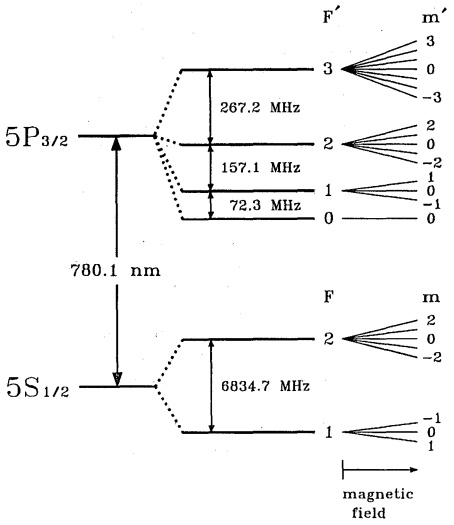
\includegraphics[width=0.45\textwidth]{plots/splitting_diagram.jpeg}
\caption{Energy levels of a Rubidium atom showing the nuclear states, hyperfine and Zeeman splittings. The difference in energy level of each interaction is many orders of magnitude smaller than the energy difference resulting from the interaction on its left. (Image Source: The Optical Society)}
\label{splitting}
\end{figure}
In Fig. \ref{splitting}, we can see that the fine structure, hyperfine, and Zeeman interactions splits the energy levels into j , f and $m_f$ levels respectively. The goal of the optical pumping is to ``pump" the atoms into the m=1/2 state. This is achieved by sending in radio frequency field (RF) to induce transition from the ground state ($S_{1/2}$) to the $P_{1/2}$ state. Compared to the transition level energy difference, the splitting of magnetic field energies is smaller by many orders of magnitude smaller, so the spread of energy of the light is sufficient to bring the atom up to the $m_F $= 1 state~\cite{Paschotta}.  Then the excited atoms undergoes spontaneous emission where they decay down to the $S_{1/2}$ state with a 50\%-50\%  probability of landing on the $m_F $= 0 and 1 levels. The  $m_F $= 0 atoms are again pumped up by the RF and then fall down to the  $m_F $= 0 and 1 levels. As many iterations of this cycle occurs, the atoms are ``stacked" up to the  $m_F $= 1 level and we have successfully pumped all the atoms onto that level.
\section{Apparatus and Procedure}\label{sec:ap}
%Apparatus and Procedure: You should have enough detail so that one familiar with physics but not with the particular experiment at hand could reproduce your experiment if necessary. A block diagram of the equipment is essential here—this should be your own, and not copied out of a book or lab manual. Explain the major pieces of equipment and what they do, but do not overwhelm your reader with details here!
\begin{figure}[h]
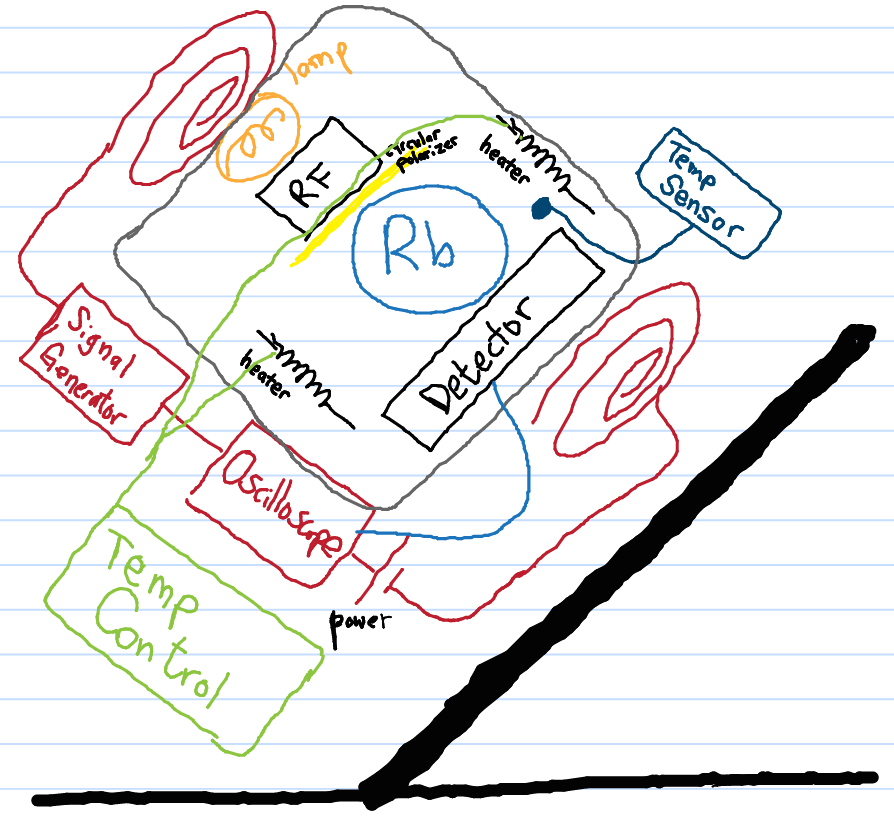
\includegraphics[width=0.45\textwidth]{plots/setup.png}
\caption{Optical pumping experimental setup. Helmholtz coil and the bulk of the experiment is tilted so that the magnetic field vector adds with the Earth's magnetic field.}
\label{setup}
\end{figure}
\paragraph{Instrumentation} Most of the experimental apparatus is placed inside a metal box so that the heating can be directly applied to Rubidium atoms. There is a circular  polarizer in front of the light source  to ensure that the angular momentum of the incident light is $\hbar$, since circularly polarized light can only change the angular momentum by $\Delta m = 1$. This circularly polarized light passes through the Rubidium gas bulb. The Rubidium gas bulb contains both Rb-85 and Rb-87 isotopes which have nuclear moments of I = 5/2 and I=3/2 respectively. 
The magnetic field given by the Helmholtz coil depends on how much current is passing through the coils, a variable that we are varying in our experiment, as shown by Eq.\ref{currentB}.
\begin{equation}\label{currentB}
B_{H} = 0.9\times 10^{-6} \frac{T\cdot m}{A} \frac{N i}{a}
\end{equation}
\paragraph{Procedures}
First, we heat up the sample and make sure that it does not exceed \footnote{Contrary to the temperature sensor's display, the temperature is measured in Fahrenheits rather than Celsius.}. Using the settings given on the lab manual, we additionally sweep through a freqeuncy  range adjust the resolution settings  until we see a resonance curve on the oscilloscope. Then, we switch the oscilloscope from the default time series mode to the X-Y mode to observe a Lissajous figure. There may be minor fluctuations to the signal due to temperature fluctuations.We measure the minimum and maximum current value ($I^+$, $I^-$) that still yields a symmetric Lissajous curve and make this the error range of our current measurement, since within this range, we can not determine what is the best value corresponding to the resonant frequency. The errors determined by the $I^+$, $I^-$ ranges is propagated through our subsequent analysis in Sec. \ref{sec:analysis} and to get an error estimate on the final computed value of Earth's magnetic field. 
\par We repeat this procedure to obtain more measurements by setting a different magnetic field strength (by changing the current) and varying the frequency to find the new resonant frequency. Then we change the direction of the magnetic field and take another set of measurements. To find the resonant frequency for the other species, we need to change the frequency and make sure that the resonance occur at a different frequency as the first species that we were measuring and again repeat the data measurement procedure for this species.
 \begin{figure}[h]
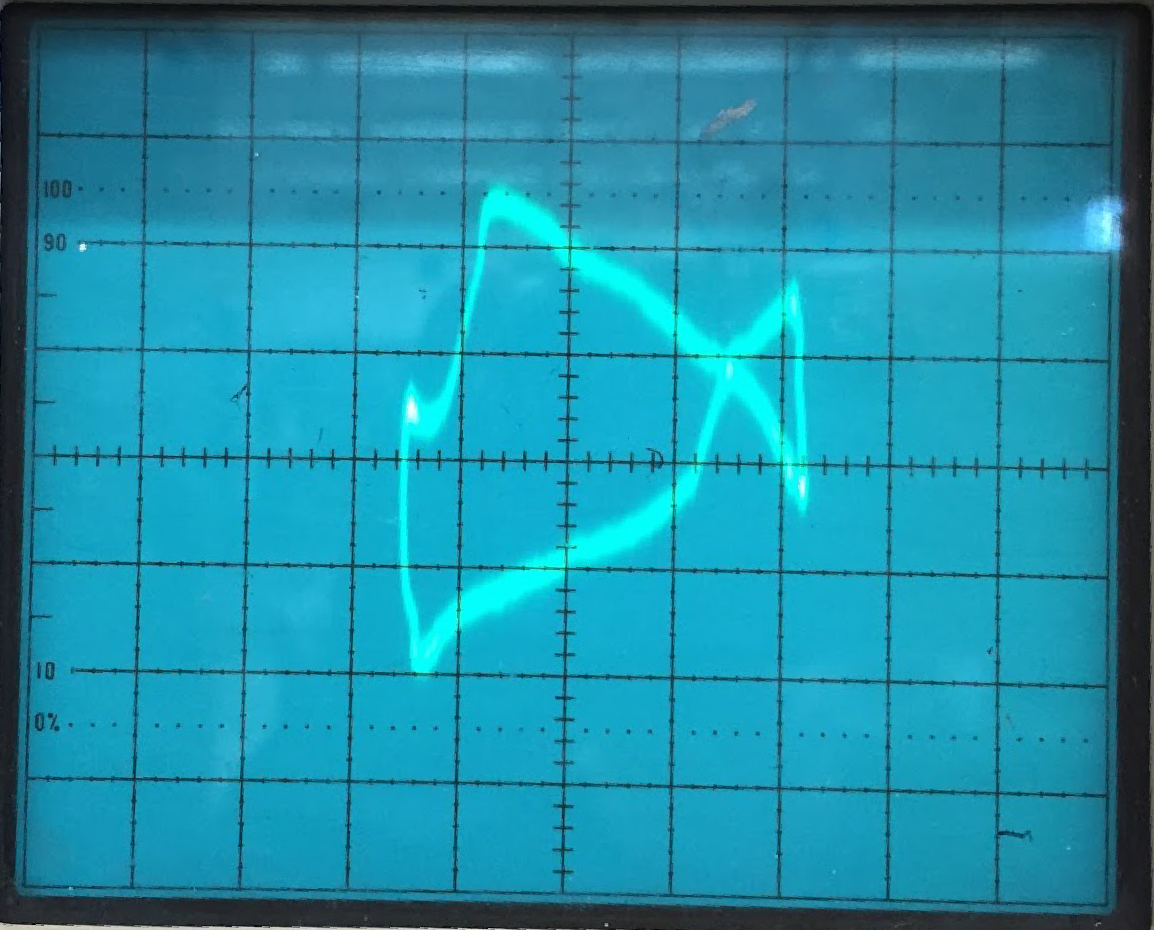
\includegraphics[width=0.45\textwidth]{plots/curve_pic.png}
\caption{An example of a assymetrical Lissajous figure measured at zero current.}
\label{lissa}
\end{figure}
\section{Analysis}\label{sec:analysis}
%Analysis:  the calculations that the lab manual asks you to do are supposed to act as a guide to your analysis, and not as a series of separate calculations. agree with prediction? error analysis? source of error, uncertainty?  
\paragraph{Determining Nuclear Moments of Observed Species}
\par By taking the ratio of the Breit-Rabi equation for the two species: 
\begin{equation*}
\frac{\frac{\nu_1}{B_1} = \frac{2.799}{2I_1+1}}{\frac{\nu_2}{B_2} = \frac{2.799}{2I_2+1}} = \frac{2I_2+1}{2I_1+1}
\end{equation*}
\begin{equation*}
\frac{\nu_1}{\nu_2} = \frac{B_1}{B_2}\Bigg(\frac{2I_2+1}{2I_1+1}\Bigg)
\end{equation*}
We chose the ``best" value of $\frac{\nu_1}{\nu_2} $ as one and this yielded a 2I+1 ratio of about 2/3. Since we know that nuclear moments must be half integer values, we can confidently round up our result to the closest half integer. We can also  deduced that if Species 1 was Rb-85 (I=5/2) and Species 2 was Rb-87 (I = 3/2) ~\cite{PhysRev}, then we would get the appropriate 2I+1 ratio. The errors on these deduced values are accurate to 3 significant figures, because the only uncertainty is on the numerical coefficient 2.799. 
\par Knowing the $I_1$ and $I_2$ values, we can use the Breit-Rabi equation (Eq.\ref{br}) to compute the magnetic field and compare this with the one that we obtain from Eq.\ref{currentB}. For species 1, the mean square difference between the two measures of the magnetic field is 0.0915 and for species 2 the mean squared difference is 0.0973. This value gives us an estimate of the systematic error of the possible non-uniformity of the Helmholtz coil number and radius.  Using this technique, we were able to obtain a more accurate estimate of the numerical coefficient in Eq.\ref{currentB} of  $9.963\times 10^{-7}$. 
\paragraph{Data Fitting and Transformation}
\par We perform a linear regression using Python's \texttt{polyfit} function on the data using the model obtained from rearranging the Breit-Rabi equation into the linear form (y = ax+b), where the frequency is the dependent variable and the magnetic field strength is the independent variable.
\begin{figure}[h]
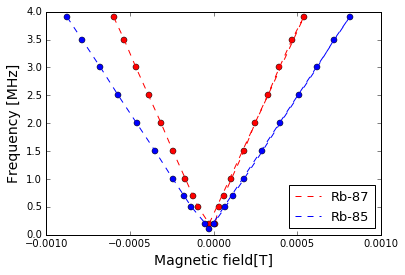
\includegraphics[width=0.45\textwidth]{plots/all_data.png}
\caption{Experimental data of magnetic field strength of Helmholtz coil versus resonant frequency before data transformation.}
\label{linear_fit}
\end{figure}
\par In order to decrease the error on the parameters for linear regression, we flipped the negative data along the x axis so that we could perform two linear fits so that we have double the size of the sample. The error estimates on the parameters can be obtained from the derivation of the  maximum log-likelihood estimator on a linear regression model ~\cite{num_rec}:
\begin{equation}
\sigma_a ^2 = S_{xx}/\bigtriangleup
\sigma_b^2 = S/\bigtriangleup
\end{equation}
where $\bigtriangleup = SS_{xx}-(S_x)^2$,$ S_{xx} = \sum^N_{i=1}\frac{x_i^2}{\sigma_i^2}$, $S_x = \sum^N_{i=1}\frac{x_i}{\sigma_i^2}$, $S =\sum^N_{i=1}\frac{1}{\sigma_i} $.
With this error estimate,  we summarize the fitting coefficients and their respective errors in Table. \ref{fitting_coefficients}.
\begin{table}[]
\centering
\caption{Fitting coefficients on the experimental data, where a is the slope and b is the y-intercept. }
\label{fitting_coefficients}
\begin{tabular}{lllll}
Species & a       & b      & $\sigma_a$ & $\sigma_b$ \\
Rb-85   & 4644.29 & 0.1342 & $1.091\times 10^{-6}$ & 0.231     \\
Rb-87   & 6983.93 & 0.2069 & $1.201\times 10^{-6}$ & 0.573    
\end{tabular}
\end{table}
We obtained a chi squared value of 3.571 for Rb-85 and 3.724 for Rb-87. The chi squared goodness-to-fit test shows that the experimental values are very close to the modelled values (p<0.01) and with the values of nuclear spins found in our analysis.
\begin{figure}[h]
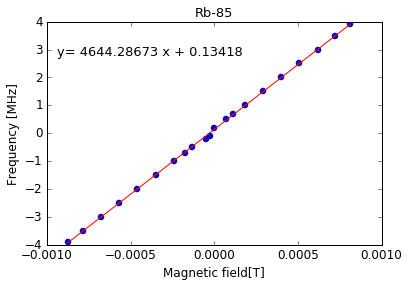
\includegraphics[width=0.45\textwidth]{plots/rb85.png}
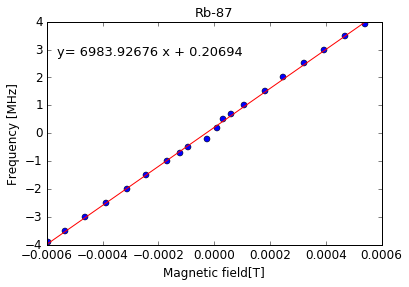
\includegraphics[width=0.45\textwidth]{plots/rb87.png}
\caption{This is the linear regression on the experimental data for Rb-85 and Rb-87. The error bar is too small compared to the pixels spanned by the datapoint, so it can not be seen on this plot.}
\label{linear_fit}
\end{figure}
\paragraph{Estimating Earth's magnetic field}
\par At the zero current point, the magnetic field is zero, so there is no magnetic field contribution from the Helmholtz coil so $B_{total} = B_{earth}$. This could also be thought of as the y intercept of the linear regression: 
$$ B_H = \frac{(2I+1)}{2.799} \nu - B_e $$.
From the two species, we obtained two estimates of the total magnetic field as $59.28\pm 9.151 \mu T $ for species 1 and $91.428  \pm 9.72 \mu T$, yielding a average value o f$75.354\pm 9.72 \mu T $ . The actual magnetic field strength in Berkeley is 48.6$\mu T$,according to Wolfram Alpha. This discrepancy can not be completely accounted for by the error on our recorded measurement. Possible sources error may include instrumentation systematics, non-uniformity of the magnetic field and electronics reading noise. 
\section{Conclusion}\label{sec:conclusion}
%findings, future improvement? 
 In this experiment, we performed the technique of optical pumping to populate $m_F=1$ level of the Rubidium atom. We obtained the resonance frequencies of the two species and used their ratios to determine the nuclear moments of Rb-85 (I=5/2) and Rb-87(I=7/2). Given these current measurements, we also able to attain a more precise numerical coefficient in the current-field relation of $B_{H} = 9.963\times 10^{-7}\frac{T\cdot m}{A} \frac{N i}{a}$.We perform a linear regression to fit the data to the Breit-Rabi equation with a p<0.01 goodness of fit. Using the y-intercept of the magnetic field versus frequency plot, we can determine the magnetic field of the Earth as $75.354\pm 9.72 \mu T$. This field strength measurement demonstrates the applicability of the optical pumping technique as weak field magnetometers. Sources of error in our experiment include non-uniformity of the magnetic field from the Helmholtz coil and the uncertainty in the range of currents that yields a symmetrical Lissajous figure. As we can see in Fig. \ref{linear_fit}, the residual (deviation from the regression) is largest near values close to zero, if we were given more time on this experiment, possible future directions includes taking more measurements in regions that are close to zero current, to better constrain the fitting coefficients and therefore obtain a more precise measurement of the Earth's magnetic field. 
\section*{Acknowledgments}
I am sincerely thankful for support from Professor Harmut Haeffner, Kam-Biu Luk, Don Orlando, and my lab partner Xiyue Wang for contributing to successful completion of this lab.
\bibliographystyle{SIGCHI-Reference-Format}
\bibliography{sample}

%Raw Data: You must include the data that you took in lab in an appendix; the data should be clear enough so that someone could look at it and determine what you measured and how you measured it. You should be keeping a lab notebook, so simply photocopy all relevant pages. Your report should include all of the listed sections, along with the signed Pre-lab and Mid–Lab Discussion sheets.

\end{document}


